\documentclass[a4paper]{article}
\usepackage[utf8]{inputenc}
\usepackage[francais]{babel}
\usepackage[babel=true]{csquotes}
\usepackage{graphicx}

\pagestyle{headings}

\title{Programming techniques : Project 2}
\author{Marien Bourguignon \& Raphaël Javaux}
\date{}

\begin{document}

\maketitle

    \paragraph{} My solution for this project consists in an efficient 
sort-based algorithm which is able to turn a random polygon into a simple one
in quasi-linear time.

    \paragraph{Algorithm} The idea of my algorithm is to (1) select the 
leftmost point and (2) sort the remaining points according to their slopes over
the leftmost point. This way, no pair of edges will ever cross each-other.
The following figure shows the leftmost point in red and the new polygon's order
in green with the ascending slope in grey :

    \begin{figure}[h]
        \centering
        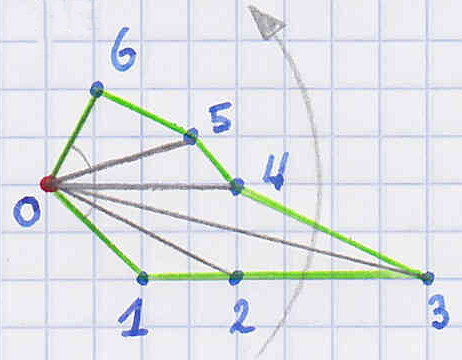
\includegraphics{schema.jpg}
    \end{figure}

    \paragraph{Slope vs. polar coordinates} Another way to sort points is to
compare them by their angles instead of their slope. This doesn't require you to
find the leftmost point, but comparisons are slower because you need to compute
expensive trigonometric functions.

    Moreover, when comparing slopes with positive x-coordinates (as they always
are, because of the leftmost point), you are able to replace this comparison:
$\frac{dy_1}{dx_1} < \frac{dy_2}{dx_2}$ by this comparison : 
$dy_1 * dx_2 < dy_2 * dx_1$.

    This is relevant to remove divisions because multiplications are eight times
faster on modern CPUs.

     \paragraph{Complexity} As the comparison of two points by their slopes runs
in constant time, the complexity of the algorithm is only relative to that of
the QuickSort algorithm, so this solution runs in $O(N * log (N))$ on average
(the complexity of the leftmost point has been removed as it grows slowly).

    The algorithm consumes a constant memory space as it runs in place.

\end{document}